\chapter{Alberi decisionali}
%%%%%%%%%%%%%%%%%%%%%%%%%%%%%%
Vediamo come sfruttare una struttura dati discreta, l'\textbf{albero di
  decisione}, per affrontare problemi di \textit{concept learning}. Su questa
struttura implementeremo l'algoritmo chiamato \textbf{ID3} che tra le ipotesi
sceglie il risultato dell'apprendimento tramite esempi di addestramento. La
lista delle ipotesi in questo caso è enorme e la scelta è guidata dal cosiddetto
\textit{information gain}.
\section{Alberi di decisione come elementi esecutivi}
\begin{definizione}
Un albero di decisione prende in input un oggetto o una situazione descritta da un insieme di \textbf{attributi} e restituisce una \textit{"decisione"}, ovvero il valore predetto di uscita per tale input.
\end{definizione}
Gli attributi dell'input possono essere discreti o continui sebbene in questo libro ci limiteremo a studiare i casi discreti. L'apprendimento di una funzione a valori discreti viene chiamata \textbf{classificazione}, mentre nel caso continuo \textbf{regressione}. In particolare ci concentreremo sulla classificazione \textbf{booleana}, dove ogni esempio è classificato come vero o falso.\\  Un albero di decisione funziona eseguendo in sequenza una serie di test, dove \textbf{ogni nodo} interno all'albero corrisponde a un test sul valore di una delle proprietà, e le diramazioni uscenti dal nodo sono etichettate con tutti i possibili risultati. Ogni foglia specifica il valore da fornire in uscita. Lo scopo è quello di apprendere una definizione del \textbf{predicato obiettivo}. Se vogliamo esprimere un problema come un problema di apprendimento, per prima cosa dobbiamo definire gli attributi disponibili per descrivere gli esempi del dominio (proprio come abbiamo fatto durante il Concept Learning).\\
In figura \ref{dt} si ha un esempio dove si hanno attributi che hanno anche più di due valori. In rosso si hanno gli
attributi, in blu i valori degli attributi e in arancione le foglie con i
risultati. Le foglie sono le risposte booleane.
\section{Espressività degli alberi di decisione}
Ogni particolare ipotesi per un albero di decisione del \textbf{predicato obiettivo} preposto può essere vista come un'asserzione nella forma:
\[\forall s\,\,\, PredicatoObiettivo(s)\,\,\,\iff\,\,\,(P1(s)\vee P2(s)  \vee ... Pn(s))\]
Dove ogni condizione $P_H(s)$ è una congiunzione di test corrispondente a un cammino dalla radice dell'albero a un nodo foglia con esito positivo.
Possiamo quindi scegliere, al posto delle classiche funzioni booleane,
\textbf{alberi di decisione} per rappresentare un modello che applicato ad
esempi non visti ci dirà se applicare in output un'etichetta vera o falsa in
base a quanto appreso. Siamo in ambito di \textbf{apprendimento
  supervisionato}.Possiamo dire che gli alberi decisionali descrivono tutte le funzioni booleane (figura \ref{dt2} e figura \ref{dt3}). 
Notiamo a questo punto come l'albero decisionale in figura \ref{dt} è la
rappresentazione di:
\[(Outlook=Sunny\,\land\, Humidity=Hight)\]
\[\lor(Outlook=Overcast)\]
\[\lor(Outlook=Rain \land Wind=Weak) \] \\ Avendo $n$ funzioni booleane avremo un numero distinto di tabelle diverità (e quindi di alberi decisionali), ciascuna con $2^n$ righe, pari a $2^{2^{n}}$. In altre parole, gli alberi decisionali vanno bene per alcuni tipi di funzione e non per altri.\\
  \textbf{NOTA:} non esiste alcuna funzione booleana che non possa essere scritta sotto forma di un albero di decisione.\\
\begin{figure}
  \centering
  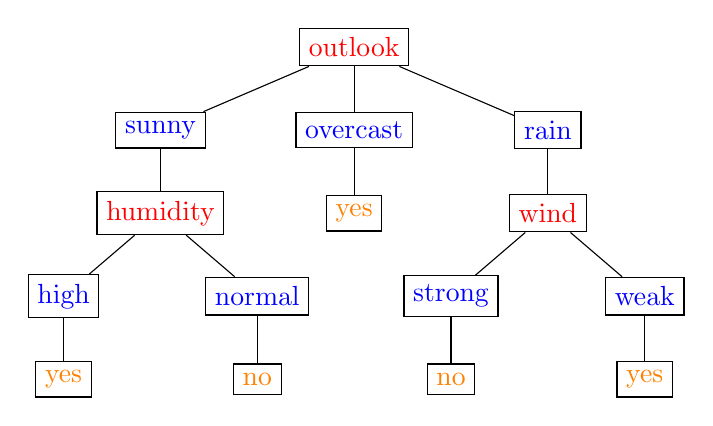
\begin{tikzpicture}[nodes={draw}, -, sibling distance=70pt, level
      distance=30pt]  
      \node{\color{red} outlook}
      child {node {\color{blue} sunny}
        child{node {\color{red} humidity}
          child{node {\color{blue} high}
            child{node {\color{orange} yes}}}
          child{node {\color{blue} normal}
            child{node {\color{orange} no}}}}}
      child {node {\color{blue} overcast}
        child {node {\color{orange} yes}}}
      child {node {\color{blue} rain}
        child{node {\color{red} wind}
          child{node {\color{blue} strong}
            child{node {\color{orange} no}}}
          child{node {\color{blue} weak}
            child{node {\color{orange} yes}}}}};
    \end{tikzpicture}
  \caption{Esempio di albero decisionale}
  \label{dt}
\end{figure}

\begin{figure}[H]
  \centering
  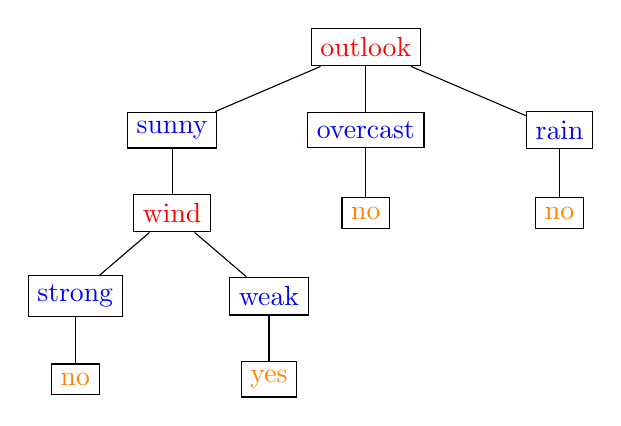
\begin{tikzpicture}[nodes={draw}, -, sibling distance=70pt, level
    distance=30pt]  
    \node{\color{red} outlook}
    child {node {\color{blue} sunny}
      child{node {\color{red} wind}
        child{node {\color{blue} strong}
          child{node {\color{orange} no}}}
        child{node {\color{blue} weak}
          child{node {\color{orange} yes}}}}}
    child {node {\color{blue} overcast}
      child {node {\color{orange} no}}}
    child {node {\color{blue} rain}
      child{node {\color{orange} no}}};
  \end{tikzpicture}
  \caption{Esempio di albero decisionale per la formula $(Outlook=Sunny)\land
    (Wind=Weak)$} 
  \label{dt2}
\end{figure}
\begin{figure}[H]
  \centering
  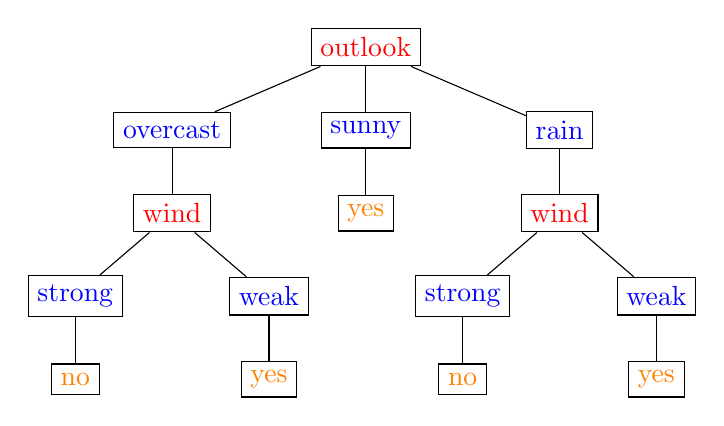
\begin{tikzpicture}[nodes={draw}, -, sibling distance=70pt, level
    distance=30pt]  
    \node{\color{red} outlook}
    child {node {\color{blue} overcast}
      child{node {\color{red} wind}
        child{node {\color{blue} strong}
          child{node {\color{orange} no}}}
        child{node {\color{blue} weak}
          child{node {\color{orange} yes}}}}}
    child {node {\color{blue} sunny}
      child{node {\color{orange} yes}}}
    child {node {\color{blue} rain}
      child{node {\color{red} wind}
        child{node {\color{blue} strong}
          child{node {\color{orange} no}}}
        child{node {\color{blue} weak}
          child{node {\color{orange} yes}}}}};
  \end{tikzpicture}
  \caption{Esempio di albero decisionale  per la formula $(Outlook=Sunny)\lor
    (Wind=Weak)$}
  \label{dt3}
\end{figure}
\section{Introduzione di alberi di decisione dagli esempi}
Un esempio per un albero di decisione booleano consiste in un vettore di attributi in input, $X$, e un singolo valore booleano in output $y$: ovvero un \textbf{Training Set} (come quello visto nel precedente capitolo).
Il problema di trovare un albero decisionale che si accorda con l'insieme di addestramento potrebbe sembrare difficile, ma in effetti esiste una soluzione banale: possiamo semplicemente costruire un albero che ha un cammino verso una foglia per ogni esempio, e lungo il cammino verificare ordinatamente il valore di ogni attributo ed eseguire il valore dato nell'esempio. Il problema di questo albero è che si limita a \textbf{memorizzare} le osservazioni senza estrarre dagli esempi alcuno schema, per cui non ci possiamo aspettare che sia capace di estrapolare soluzioni che non ha già incontrato. Per evitare queste problematiche ricorriamo all'algoritmo \textbf{ID3}: verificare per primo il valore dell'attributo più "significativo", ovvero quello che ha il maggiore impatto sulla classificazione. In questo modo cerchiamo di arrivare a una soluzione in un numero ridotto di test, ovvero: creare un albero più piccolo ma equivalente logicamente. In generale, dopo che il test del primo attributo suddivide gli esempi, ognuno dei suoi esiti può essere considerato un problema di apprendimento completamente nuovo, con un attributo in meno e un insieme di esempi più piccolo. Possiamo perciò identificare quattro casi:
\begin{itemize}
    \item Se ci sono esempi sia positivi che negativi, scegliamo l'attributo che li suddivide meglio.
    \item Se tutti gli esempi rimanenti sono positivi \textbf{o} negativi, abbiamo finito: possiamo rispondere Y o N rispettivamente agli esempi.
    \item Se non riesco a classificare alcun esempio, allora non è stata osservata alcuna situazione con quei valori di attributi. Restituiamo un valore di default.
    \item Se non rimane alcun attributo ma ci sono ancora esempi sia positivi che negativi, significa che tali esempi hanno esattamente la stessa descrizione (di valori sugli attributi) ma classificazione diverse. Questo può accadere quando alcuni dati sono scorretti, ovvero c'è \textbf{rumore} (vedremo in seguito come occuparcene).
\end{itemize}
\subsection{Rappresentazione degli alberi}
Ricordiamo che un albero decisionale è formato da:
\begin{itemize}
  \item \textbf{Nodes (\textit{nodi})}: etichettati da i vari attributi.
  \item \textbf{Branches \textit{rami}}: etichettati con i possibili valori
  dell'attributo che etichetta il nodo sorgente del ramo.
  \item \textbf{Leef nodes (\textit{foglie})}: etichettati con gli outcome della
  previsione.
\end{itemize}
Un percorso dalla radice fino alla foglia mi rappresenta una congiunzione di
attributi mentre l'albero in se è una disgiunzione di congiunzioni, una
per ogni percorso radice-foglia. Un albero formalizza la congiunzione di
vincoli su attributi ma può estendere il linguaggio per accettare delle disgiunzioni di vincoli su questi ultimi.\\
Usando funzioni booleane \footnote{un attributo può avere valore $\top,\,\,\, T$ o
$\bot,\,\,\, F$} posso convertire tabelle di verità in alberi decisionali, avendo ogni percorso dalla radice a una foglia che rappresenta una
\textbf{regola}, e l'intero albero rappresenta la congiunzione di tutte le
regole. Le foglie quindi sono gli assegnamenti di verità della tabella.\\ 
Posso avere alberi diversi a seconda della scelta del nodo radice.\\
\begin{esempio}
  Vediamo i due alberi per la funzione booleana $\lor$ e $\oplus$.\\
  La seguente tabella e le figure \ref{OR decision tree} e \ref{XOR decision tree} ne mostrano le informazioni.
  \begin{table}[H]
    \centering
    \begin{tabular}{c|c|c|c}
      $A$ & $B$ & $A\lor B$ & $A\oplus B$ \\
      \hline
      $T$ & $T$ & $T$ & F\\
      $T$ & $F$ & $T$ & T\\
      $F$ & $T$ & $T$ & T\\
      $F$ & $F$ & $F$ & F
    \end{tabular}
  \end{table}
  
  \begin{figure}[h]
    \centering
    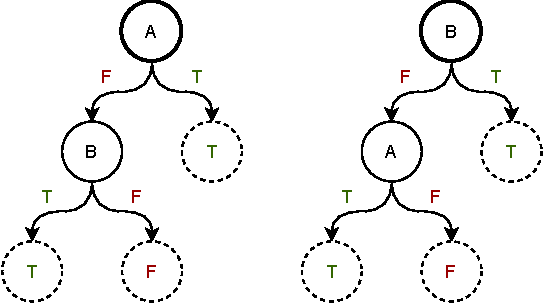
\includegraphics[scale = 0.9]{img/dt1.pdf}
    \caption{OR decision tree}
    \label{OR decision tree}
  \end{figure}
 
  \begin{figure}[h]
    \centering
    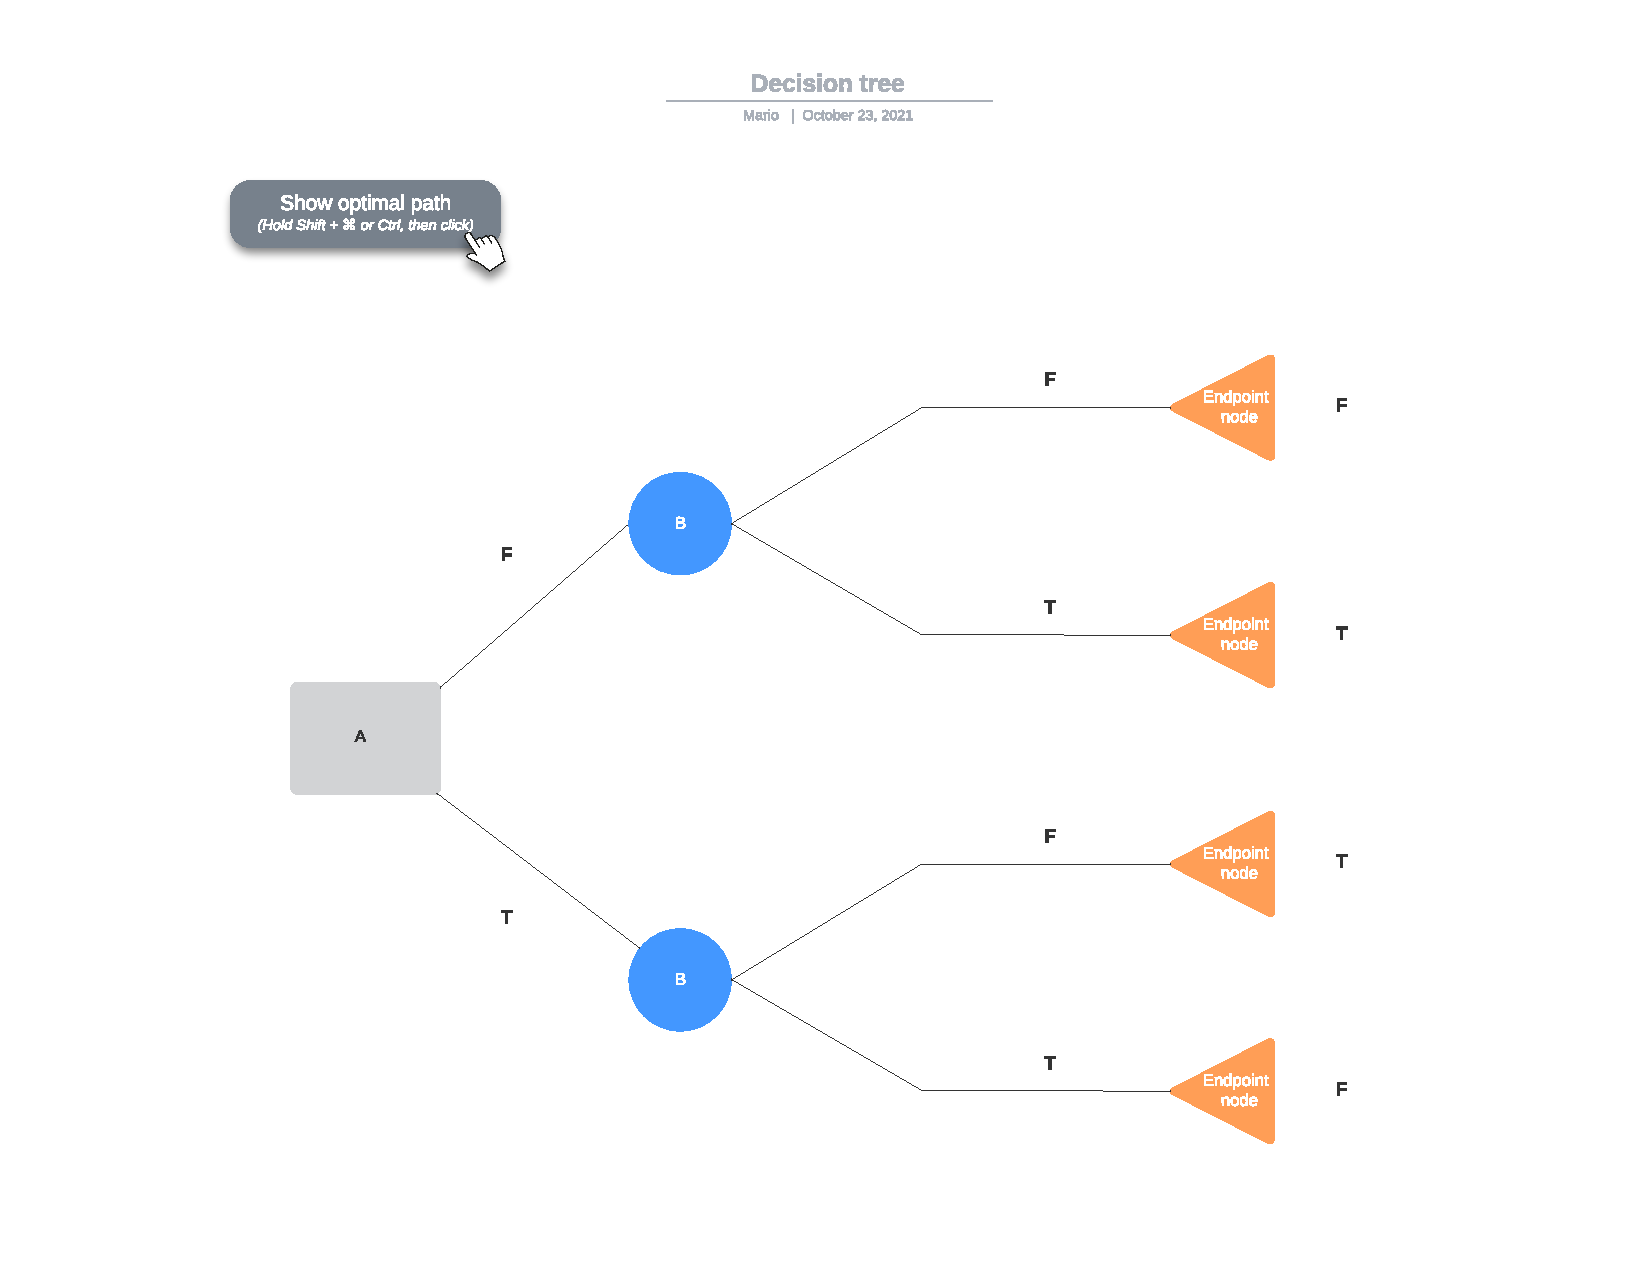
\includegraphics[scale = 0.5]{img/XOR.pdf}
    \caption{XOR decision tree}
    \label{XOR decision tree}
  \end{figure}
\end{esempio}
Essendo sempre nel concept learning, nel caso di funzioni booleane, anche il
target è booleano.
Gli alberi di decisione possono essere utilizzati anche nel continuo, per attributi numerici.
\begin{esempio}
  Immaginando  di non ritrovarci più in casi discreti ma di passare a casi \textbf{continui}. Prendiamo le istanze definite da due attributi, $x$ e $y$ e costruisco un
  albero di decisione che definisce in quali aree del piano ho $-$ e quali ho
  $+$.
  \newpage
  Si ha il seguente piano (\textbf{sull'asse delle $y$ il primo valore a partire
  dall'origine è un cinque non un sette}): 
  \begin{figure}[H]
    \centering
     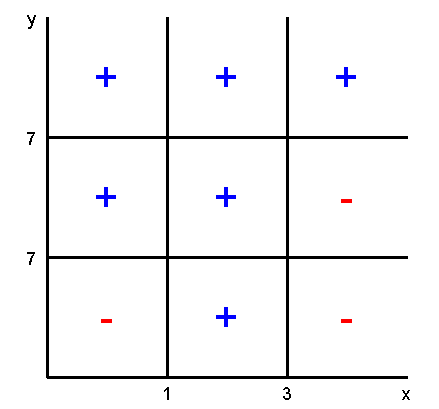
\includegraphics[scale = 0.8]{img/dt3.pdf}
  \end{figure}
  E si ottiene, per esempio, il seguente albero decisionale:
  \begin{figure}[H]
    \centering
    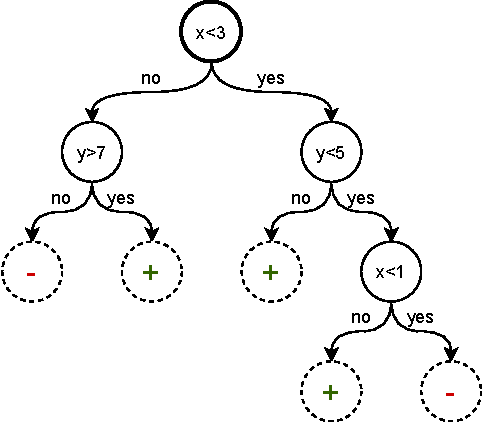
\includegraphics[scale = 0.9]{img/dt4.pdf}
  \end{figure}
  Dove a ciascun nodo è associata una condizione e agli archi il fatto che sia
  verificata o meno.\\
  Si nota come non si hanno tutte le condizioni, infatti, per esempio, con $x>3$
  mi basta $y>7$ per trovare il $+$ e $y<7$ per il $-$ (non dovendo andare
  specificatamente a guardare anche $y<5$ o $y>5$).\\
  \textbf{Quello disegnato è solo uno dei possibili alberi.}
\end{esempio}

\subsection{Algoritmo ID3}
Vista la difficoltà di scegliere l'albero si ha l'idea di scegliere un piccolo
albero di partenza (o più piccoli) e ricorsivamente l'attributo più
significativo (sia nei nodi rossi intermedi che nelle foglie) come radice per il
sotto-albero. Si fanno quindi crescere in modo 
coerente gli alberi piccoli scelti in partenza. Si punta ad arrivare a un
albero valido per tutti gli esempi ricevuti e anche per quelli non visti.\\
\begin{algorithm}[H]
  \begin{algorithmic}
    \Function{ID3}{esempi, attrib, default}
    \If{esempi è vuoto return default}
    \EndIf
    \If{tutti gli \textit{esempi} hanno la stessa classificazione \textbf{return la classificazione}}
    \EndIf
    \If{\textit{attrib} è vuoto \textbf{return VALORE\_MAGGIORANZA(esempi)}}
    \EndIf
    \State $best \gets$ \textit{il ``miglior'' attributo di decisione per il
    prossimo nodo}
    \State $albero \gets$ \textit{un nuovo albero di decisione con alla radice \textbf{best}}
    \State $m \gets$ \textit{VALORE\_MAGGIORANZA(esempi)}
    \For {\textit{ogni valore $V_i$ dell'attributo best}}
    \State $esempi \gets$ \textit{Elementi di esempi con $best = Vi$}
    \State $sottoAlb \gets$ \textit{ID3(esempi, attrib-best, m)}
    \State \textit{Aggiungi un ramo all'albero con etichetta $V_i$ e sottoalbero \textbf{sottoalb}}
    \EndFor
    \State \textit{\textbf{return albero}}
    \EndFunction
  \end{algorithmic}
  \caption{Algoritmo ID3 (Iterative Dichotomiser 3)}
\end{algorithm}
Facciamo qualche osservazione finale sull'\textbf{algoritmo ID3}:
\begin{itemize}
  \item Lo spazio delle ipotesi è completo e sicuramente contiene il target.
  \item Ho in output una singola ipotesi.
  \item Non si ha backtracking sugli attributi selezionati, si procede con una
  ricerca greedy, trovando scelte buone localmente ma non ottime.
  \item Fa scelte basate su una ricerca statistica, facendo sparire incertezze
  sui dati.
  \item Il bias non è sulla classe iniziale, essendo lo spazio delle ipotesi
  completo, ma sulla scelta di solo alcune funzioni, preferendo alberi corti (e
  più semplici) e posizionando attributi ad alto information gain vicino alla
  radice. Il bias è quindi sulla preferenza di alcune ipotesi. Si usa il
  criterio euristico di \textit{rasoio di Occam}.
  \item $H$ è l'insieme potenza delle istanze $X$.
\end{itemize}
Sfortunatamento un algoritmo scritto in questo modo è destinato a compiere qualche errore, il nostro compito sarà quello di \textbf{scoprire quanto sara scorretto}.
\section{Scegliere L'insieme degli attributi}
Ricordiamo che l'idea è quella di minimizzare la profondità dell'albero risultante. L'idea è scegliere l'attributo che fornisce la classificazione più esatta possibile degli esempi.
Bisogna in primis capire cosa si intende come \textbf{attributo migliore}.
Gli esempi positivi sono gli esempi che già mi hanno restituito \textit{yes} mentre quelli negativi sono quelli che mi hanno restituito \textit{no}.
Immaginiamo di avere un insieme di esempi $y_i$ positivi e $n_i$ negativi: \[ [y_1, y_2, y_3, y_4, n_1, n_2, n_3]\]
\begin{figure}[H]
  \centering
  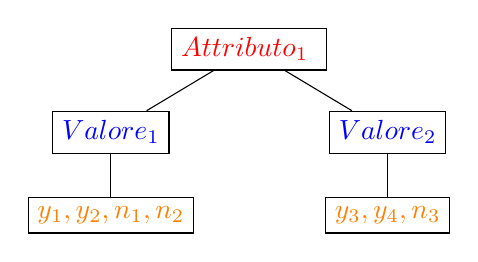
\begin{tikzpicture}[nodes={draw}, -, sibling distance=100pt, level
    distance=30pt]  
    \node{\color{red} $Attributo_1$ \color{black}}
    child {node {\color{blue} $Valore_1$}
      child{node {\color{orange} $y_1, y_2, n_1, n_2$}}}
    child {node {\color{blue} $Valore_2$}
      child{node {\color{orange} $y_3, y_4, n_3$}}};
  \end{tikzpicture}
\end{figure}
La figura soprastante nostra un albero che ha come attributo $Attributo_1$ e come possibili esiti/valori di tale attributo: $Valore_1$ e $Valore_2$. Notiamo che questo attributo non è un buon attributo, poiché suddivide gli esempi in maniera \textit{mista}: l'attributo non possiede valori per cui smistare in maniera omogenea ogni singolo esempio.
\begin{figure}[H]
  \centering
  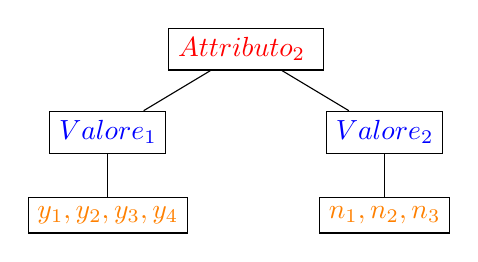
\begin{tikzpicture}[nodes={draw}, -, sibling distance=100pt, level
    distance=30pt]  
    \node{\color{red} $Attributo_2$ \color{black}}
    child {node {\color{blue} $Valore_1$}
      child{node {\color{orange} $y_1, y_2, y_3, y_4$}}}
    child {node {\color{blue} $Valore_2$}
      child{node {\color{orange} $n_1, n_2, n_3$}}};
  \end{tikzpicture}
  \label{Albero2}
\end{figure}
La figura indicata mostra invece un attributo che suddivide molto meglio gli esempi, in particolare $Valore_1$ possiede esempi positivi e $Valore_2$ esempi negativi.
\begin{definizione}
  Un attributo perfetto suddivide gli esempi in insiemi tutti positivi o tutti negativi
\end{definizione}

Ora sia Mario Avolio (autore di questa sezione di appunti) e sia voi vi chiederete "\textit{Ma come faccio a capire quanto è buono un attributo?}. In teoria la misura dovrebbe avere valore massimo quando l'attributo è perfetto e minimo quando l'attributo non è utile per nulla(tipo Windows). Una misura adeguata è la quantità attesa di \textbf{informazione} fornita dall'attributo. Essa viene misurata in \textbf{bit}. \\ Un bit d'informazione è sufficiente a rispondere $Y$ o $N$ a una domanda di cui non si sa nulla, se le possibili risposte $v_i$ hanno probabilità $P(v_i)$ allora il \textbf{contenuto informativo} $I$ della risposta corretta è dato dalla definizione di \textbf{entropia}:
\begin{definizione}
  Dato un \textbf{training set $S$} con possibili esiti sugli esempi: $v_i,\,\, i=1\ldots n$. L'entropia (fig. \ref{Entropy}) di un
  insieme di bit misura la sua quantità d'informazione (analogamente il \textbf{disordine}, ovvero il numero di elementi \textit{mischiati} tra loro, contenuto nell'insieme). In generale, se i possibili esiti $v_i,\,\, i=1\ldots n$ hanno probabilità $P(v_i)$ di essere frequenti sugli esempi, il contenuto informativo $I$ (anche chiamato \textbf{entropia}) della del training set $S$ è dato da:
  \begin{equation}
  H(P(v_1),\ldots, P(v_n))=\sum_{i=1}-P(v_i)\log_2P(v_i)
      \label{Entropy}
\end{equation}
  \end{definizione}
  \begin{figure}[H]
      \centering
      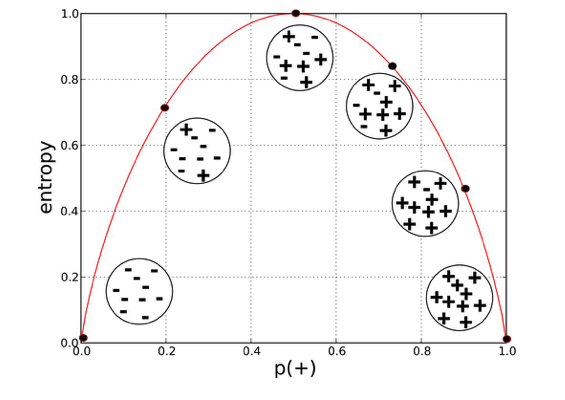
\includegraphics[width=1\textwidth]{img/entropy.png}
      \caption{Entropia al variare degli esempi \cite{}}
  \end{figure}
    Per l'apprendimento di alberi di decisione la domanda a cui vogliamo rispondere è: \textbf{dato un esempio, qual è la sua classificazione?}\\
      Per stimare la probabilità delle possibili risposte, \textbf{prima di verificare il valore degli attributi}, si può guardare la proporzione di esempi negativi e positivi nell'insieme di addestramento. Supponiamo di avere un insieme di \textbf{$p$ esempi positivi e $n$ esempi negativi}: una stima dell'informazione contenuta nella risposta corretta è:
    
      \begin{equation}
\label{Contenuto informatico di un insieme}
  I\left(\frac{p}{p+n},\frac{n}{p+n}\right)=-\frac{p}{p+n}\log_2\frac{p}{p+n}
    -\frac{n}{p+n}\log_2\frac{n}{p+n}
    \end{equation}
      
  \begin{esempio}
    Un esempio semplificato potrebbe riguardare due possibili esiti all'interno di un TrainingSet: $positivo$ e $negativo$. Se su 100 osservazioni/esempi avessimo 30 positivi e 70 negativi, allora la quantità d'informazione sarebbe:
          \begin{equation*}
  I\left(\frac{30}{100},\frac{70}{100}\right)=-\frac{30}{100}\log_2\frac{30}{100}
    -\frac{70}{100}\log_2\frac{70}{100} \approx 0.88
    \end{equation*}
  \end{esempio}

\textbf{NOTA:}
  In particolare si avrà un'alta entropia se elementi positivi e negativi sono saranno tra loro \textit{mischiati}\\
  
Il test di un singolo attributo non ci darà così tanta informazione, ma ce ne darà comunque un pò. Possiamo misurare esattamente tale quantità guardando quanta informazione ci è ancora necessaria \textit{dopo} aver effettuato il test. Ogni attributo $A$ divide l'insieme di addestramento in sottoinsiemi $E_1\dots E_v$, presupponendo che $A$ possa avere $v$ valori distinti. Ogni sottoinsieme $E_i$ ha un certo numero di esempi positivi $p_i$ e un certo numero di esempi negativi $n_i$. \\
\begin{figure}[H]
  \centering
  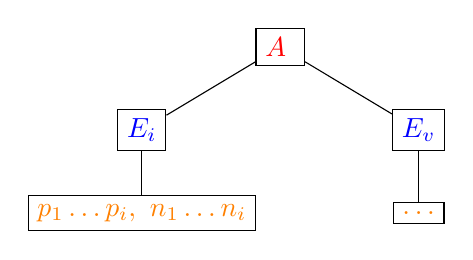
\begin{tikzpicture}[nodes={draw}, -, sibling distance=100pt, level
    distance=30pt]  
    \node{\color{red} $A$ \color{black}}
    child {node {\color{blue} $E_i$}
      child{node {\color{orange} $p_1 \dots p_i,\,\, n_1 \dots n_i$}}}
    child {node {\color{blue} $E_v$}
      child{node {\color{orange} $\dots$}}};
  \end{tikzpicture}
\end{figure}
Per cui se seguiamo una certa diramazione, per capire la classificazione di un esempio, avremo bisogno di un numero di bit \textbf{ulteriori} pari a:
\[I\left(\frac{p_i}{p_i+n_i},\frac{n_i}{p_i+n_i}\right)\]
Si faccia quindi riferimento alla regola \ref{Contenuto informatico di un insieme}. Un esempio preso casualmente dall'insieme di training avrà l'i-esimo valore per l'attributo con probabilità:
\[\frac{p_i+n_i}{p+n}\]
Ragion per cui, in media, dopo il test dell'attributo $A$, occorreranno ancora:
\begin{equation}
\label{IG Attributo}
remainder(A)=\sum_{i=1}^v \frac{p_i+n_i}{p+n}
  I\left(\frac{p_i}{p_i+n_i},\frac{n_i}{p_i+n_i}\right)
    \end{equation}
bit d'informazione per classificare l'esempio. Si noti che in questo caso verranno valutati tutti i valori distinti $v$ che $A$ può assumere. In particolare avremo $\frac{p_i+n_i}{p+n}$ di probabilità che $A$, in relazione ai propri possibili valori, distingui un determinato esempio.\\
Parliamo quindi di \textbf{information gain} $IG$ (in italiano: guadagno d'informazione) che viene calcolato su ogni
attributo $A$ e su $S$. In dettaglio il \textbf{guadagno d'informazione} ottenuto dal test dell'attributo è pari alla differenza tra il requisito informativo originale e quello corrente:
\begin{equation}
\label{IG}
IG(S, A)=I\left(\frac{p}{p+n},\frac{n}{p+n}\right)-remainder(A)
\end{equation}
\begin{definizione}
L'information gain è la riduzione aspettata nell'entropia per ordinare $S$ sull'attributo $A$. Si sceglie quindi l'attributo con il maggiore IG. 
\end{definizione} 
\textbf{NOTA:} la \ref{IG} è quindi sintetizzabile anche come:
\begin{equation}
\label{IG2}
IG(S, A)=Entropy(S)-\sum_{v\in values(A)}\frac{|S_v|}{|S|}Entropy(S_v)
    \end{equation}
\subsection{Approfondimento - Entropia di una Distribuzione di Probabilità}
% \begin{definizione}
%   Definiamo l'\textbf{entropia di una distribuzione condizionale}. Presa
%   una variabile aleatoria discreta $X$ con valori $\{x_1,\ldots, x_i\}$ 
%   hanno ciascuno probabilità $P(x_i)$, definiamo l'entropia 
% \begin{equation}
%   I_{Y|X=x_i}=-\sum_{j=1}^m P_{Y|X}(y_j|x_i)\cdot \log_2 P_{Y|X}(y_j|x_i)
%   \label{EntropiaDiUnaDistributzioneCondizionale}
% \end{equation}
% \textbf{NOTA:} la \ref{EntropiaDiUnaDistributzioneCondizionale} riprende la \ref{Contenuto informativo di un training set} utilizzando la probabilità condizionata.
% \end{definizione}
% \begin{definizione}
%   Definiamo \textbf{entropia condizionale} come il valore medio, ovvero il
%   valore atteso, dell'entropia di $p_{Y|X=x_i}$ per ciascun valore di $X$ che
%   condiziona $Y$, ovvero:
%   \[I_{Y|X}=\sum_{i=1}^n P_X(x_i)\cdot I_{Y|X=x_i}\]
%   ottenendo l'\textbf{entropia condizionale}:
%   \begin{equation}
%       H[Y|X]=\sum P(x)\cdot H(Y|X=x)
%         \label{EntropiaCondizionale}
%   \end{equation}
%   \textbf{NOTA:} essa si rifà alla \ref{IG Attributo}\\
%   \textbf{NOTA 2:} Si chiama \textbf{valore atteso} di una variabile aleatoria discreta il numero reale:
%   \[\sum_{k} P_X(X_k)\cdot X_k\]
%   Dove $X_k$ simboleggia il valore assunto dalla variabile $X$, mentre $P_X(X_k)$ è la sua densità. 
% \end{definizione}
Quando parliamo di \textit{entropia} stiamo volgendo un esperimento
concettuale. Prima dell'esperimento si ha una certa incertezza su un certo
evento, che sparisce, con sorpresa, una volta eseguito l'esperimento se l'evento
accade. D'altro canto qualora accadesse un evento atteso siamo meno sorpresi del
fatto (chiaramente perché sarebbe appunto "atteso"). Nel primo caso però si ritiene di ottenere molta informazione, nel
secondo caso poca. Come se ponessimo in una vasca quattro palline rosse, non
sarei stupito di estrarne una rossa, essendo quello che mi aspetto. D'altro
canto se ne aggiungo quattro verdi l'estrazione sarà inattesa e quindi più
interessante.\\ 
Si cerca un modo di quantificare questa ``sorpresa''. Riprendendo l'esempio
delle palline posso dire che nel primo caso (solo rosse) ho \textbf{bassa
  entropia/basso contenuto informativo} e nel secondo caso (palline miste) \textbf{alta entropia/alto contenuto informativo}. Un caso
intermedio sarebbe a \textbf{media entropia}.\\
Sia $P(x)$ la probabilità che avvenga un evento $x$ e sia $H(p)$ l'informazione (entropia) che ottengo dopo che l'evento si è verificato:
\begin{itemize}
  \item $P(x)=1\to H(p)=0$
  \item $P(x)=0\to H(p)=\infty$
\end{itemize}
L'informazione $H(p)$ e quindi una quantità non negativa:
\[H(p)\geq 0\]
Definiamo quindi l'informazione, detta anche \textit{self-information}, per un
evento $E$: 
\[H(E)=-\log_2(P(E))\]
Inoltre si può affermare che essa disponga della proprietà additiva se gli eventi sono indipendenti, ovvero:
\[H(p_1, p_2)=H(p_1)+H(p_2)\]

  L'\textbf{entropia}, definita da Claude Shannon (e quindi spesso chiamata
  \textbf{entropia di Shannon}), è l'informazione media associata ad
  una distribuzione di probabilità.\\
\begin{definizione}
Sia $X$ una variabile aleatoria che può assumere valori pari a ${x_1 \dots x_n}$ con probabilità $p_i$ analogamente a quanto detto nel precedente paragrafo possiamo calcolarne l'\textbf{entropia}, ovvero il \textbf{contenuto informativo}:
\begin{equation}
    H[X]=-\sum_{i=1}^n p_i\cdot\log_2 p_i
\label{EntropiaVariabile}
\end{equation}
\end{definizione}
Analogamente a quanto visto per un dataset, si può vedere una variabile aleatoria discreta $X$ ( quindi una distribuzione di probabilità ) come un vero e proprio dataset. Didatti si noti che la \ref{EntropiaVariabile} è identica alla \ref{Entropy}
\subsubsection{Entropia Condizionata}
Analogamente a quanto visto per la \ref{EntropiaVariabile} possiamo chiaramente sfruttare una distribuzione \textbf{condizionale} di probabilità. Ovvero possiamo sfruttare la \textbf{probabilità condizionata}. Per arrivare al concetto di \textbf{entropia condizionale} di un'intera variabile aleatoria $X$ (che supponiamo possa assumere $x_n$ valori) dobbiamo passare per un concetto intermedio. I lettori di questo libro sicuramente si ricorderanno che negli scorsi paragrafi abbiamo detto che:  
\begin{displayquote}
Ogni attributo $A$ divide l'insieme di addestramento in sottoinsiemi $E_1\dots E_v$, presupponendo che $A$ possa avere $v$ valori distinti. Ogni sottoinsieme $E_i$ ha un certo numero di esempi positivi $p_i$ e un certo numero di esempi negativi $n_i$. Per cui se seguiamo una certa diramazione, per capire la classificazione di un esempio, avremo bisogno di un numero di bit \textbf{ulteriori} pari a:
\[I\left(\frac{p_i}{p_i+n_i},\frac{n_i}{p_i+n_i}\right)\]
\end{displayquote}
Analogamente ora andremo a definire l'entropia di una variabile aleatoria discreta $Y$ condizionata dall'evento $X=x_i$, ovvero dall'evento che $X$ assuma un determinato valore. In questo caso particolare $A=X$ e $E_1 \dots E_v = x_1 \dots x_i$.
\begin{definizione}
Sia $Y$ una variabile aleatoria e $X=x_i$ l'evento che la coinvolge, allora si può descrivere l'entropia come:
  \begin{equation}
    H_{Y|X=x_i}=-\sum_{j=1}^m P_{Y|X}(y_j|x_i)\cdot\log_2 P_{Y|X}(y_j|x_i)
\label{EntropiaCondizionaleParziale}
\end{equation}
\end{definizione}
Tale equazione ci permette di definire l'entropia solo nel caso in cui un \textbf{attributo} o una \textbf{variabile aleatoria} $X$ assumano un valore $x_i$. 
\textbf{L'entropia condizionale} quantifica invece la quantità d'informazione di cui si ha bisogno per descrivere l'esito di una \textbf{variabile aleatoria} $Y$ data un'\textbf{intera} variabile aleatoria $X$. In particolare essa riprende il risultato della media di $H_{Y|X=x_i}$ per tutti i possibili valori che $X$ può assumere. 
Ricordiamo ora la quantità di bit d'informazione necessari per classificare un attributo:
\begin{displayquote}
Ragion per cui, in media, dopo il test dell'attributo $A$, occorreranno ancora:
\begin{equation}
\label{IG Attributo}
remainder(A)=\sum_{i=1}^v \frac{p_i+n_i}{p+n}
  I\left(\frac{p_i}{p_i+n_i},\frac{n_i}{p_i+n_i}\right)
    \end{equation}
bit d'informazione per classificare l'esempio. Si noti che in questo caso verranno valutati tutti i valori distinti $v$ che $A$ può assumere. In particolare avremo $\frac{p_i+n_i}{p+n}$ di probabilità che $A$, in relazione ai propri possibili valori, distingui un determinato esempio.
\end{displayquote}
Forniamo una definizione equivalente mediante \textbf{l'entropia condizionale}:
\begin{definizione}
Date due variabile aleatoria discrete $X$ e $Y$, l'\textbf{entropia condizionale} di $Y$ dato $X$ è definita come la somma ponderata di $H_{Y|X=x_i}$ per ogni possibile valore di $x_i$, usando $p(xi)$ come peso:
  \begin{equation}
    H_{Y|X}=\sum_{x_i\in X} p(x_i)\cdot H_{Y|X=x_i}
    \label{EntropiaCondizionale}
\end{equation}
\end{definizione}

\section{Valutare le prestazioni dell'algoritmo di apprendimento}
\begin{definizione}
  Un algoritmo di apprendimento è buono se produce ipotesi che riescono a predire con accuratezza la classificazione di esempi mai incontrati precedentemente.
\end{definizione}
Una predizione viene valutata in relazione a un \textbf{insieme di test}. Per questo motivo solitamente è doveroso adottare tale strategia:
\begin{enumerate}
    \item Raccogliere un grande insieme di test.
    \item Dividerlo in due insiemi disgiunti: uno per l'addestramento e uno per i test
    \item Applicare l'algoritmo di apprendimento all'insieme di addestramento, generando un'ipotesi $h$ (come già visto nel precedente capitolo sul Concept Learning)
    \item Misurare la percentuale di esempi nell'insieme di test che vengono classificati correttamente da $h$.
    \item Ripetere i passi 2 e 4 con dimensioni e insiemi diverse degli insiemi di addestramento.
\end{enumerate}
Il risultato di quanto descritto è un insieme di dati che può essere elaborato per fornire la qualità media della predizione in funzione delle dimensioni dell'insieme di addestramento. Questa funzione si può tracciare su un grafico, ottenendo la \textbf{curva di apprendimento}. \\ In questo contesto è opportuno evitare ciò che viene chiamato \textbf{peeking}: \textit{andare a creare un'ipotesi (NON generale) in base a un insieme di test che viene controllato a priori (e non a posteriori come si dovrebbe fare con dei test appunto).}
\section{Rumore e sovradattamento}
\subsection{Rumore}
Come abbiamo visto precedentemente, qualora due o più esempi contenessero la stessa descrizione ma avessero descrizioni differenti, l'algoritmo \textbf{IG3} non riuscirà a trovare un albero consistente per tutti gli esempi proposti. Una semplice soluzione per risolvere il problema è quella di far restituire a ogni nodo foglia la classificazione di maggioranza per il suo insieme di esempi. Questo solitamente porta a problemi poiché l'algoritmo genera un albero consistente per tutti gli esempi considerando quei attributi \textbf{irrilevanti} per operare distinzioni spurie tra gli esempi. 
\subsection{Overfitting}
Ogniqualvolta si opera con un insieme vasto d'ipotesi occorre stare attenti a non ricadere nell'\textbf{overfitting}(sovradattamento).
\begin{definizione}
  \textit{Definizione tratta da Wikipedia.}\\
  Definiamo formalmente l'\textbf{overfitting} come l'adattamento eccessivo,
  ovvero quando 
  un modello statistico molto complesso si adatta al campione perché ha un
  numero eccessivo di parametri rispetto al numero di osservazioni. SI ha
  quindi che un modello assurdo e sbagliato può adattarsi perfettamente se è
  abbastanza complesso rispetto alla quantità di dati disponibili.\\
  Nel machine learning se il learner viene addestrato troppo a lungo il modello
  potrebbe adattarsi a caratteristiche che sono specifiche solo del training
  set, ma che non hanno riscontro nel resto dei casi quindi le prestazioni sui
  dati non visionati saranno drasticamente peggiori.\\
  L'opposto è l'\textbf{underfitting}.
\end{definizione}

Se misuro l'errore di una ipotesi
$h$ sul training set ($error_{traini}(h)$) e poi misuro l'errore di quella
ipotesi sull'intero set delle possibili istanze
$D$ ($error_D(h)$) ho che l'ipotesi $h$ va in \textbf{overfit} sul quel data set
se:
\[error_{traini}(h) < error_{traini}(h') \,\,\land
  \,\, error_D(h)>error_D(h')\]
quindi se presa un'altra ipotesi questa è migliore della prima e ha un errore
sull'intera distribuzione delle ipotesi inferiore vado in \textit{overfit}. Il
problema è che non posso sapere se esiste tale $h'$. Per evitare il problema uso
sempre il rasoio di Occam scegliendo ipotesi semplici ed evitando di far
crescere l'albero quando lo ``split'' non è statisticamente significativo. Un
altro modo è quello di togliere pezzi, all'albero, che toccano poche istanze o
pure calcolare una \textit{misura di complessità dell'albero}, minimizzando la
grandezza dell'albero e gli errori del \textit{training set}, usando il
\textbf{Minimum Description Length (\textit{MDL})}.\\
In ID3 quindi posso scegliere sia in base all'\textit{information gain} massimo
o all'\textit{entropia} minima tra gli attributi.\\
Come specificato, una metodologia semplice da poter applicare in queste situazioni riguarda la \textbf{potatura dell'albero di decisione}. Essa opera impedendo la divisione ricorsiva su attributi che non sono chiaramente rilevamenti, anche quando i dati di un determinato nodo non sono classificati in modo uniforme. I lettori di questi appunti a questo punto si chiederanno sicuramente la seguente domanda: "Mario, se l'irrilevanza di un attributo si misura in relazione alla sua informazione fornita, quanto deve valere quest'ultima per etichettare un nodo come 'irrilevante'?". Per rispondere a questa domanda possiamo ricorrere a un \textbf{test di significatività} statistico: si comincia con un'\textbf{ipotesi nulla}, ovvero che l'attributo sia irrilevante; quindi i dati vengono analizzati per calcolare quanto si discostano effettivamente dalla totale assenza di pattern nei confronti degli esempi. Se il grado di derivazione risulta improbabile, questo viene considerato un buon indizio della presenza di un pattern significativo nei dati. \\ Un'altra possibile opzione da tenere in considerazione (magari insieme alla potatura) è la \textbf{validazione incrociata}: stimare quanto bene ogni ipotesi potrà predire dati mai incontrati.
\section{Esercizi Guidati}
\begin{esempio}
  Suppongo di lanciare una moneta, si ha:
  \[P(testa)=P(croce)=\frac{1}{2}\]
  Definiamo che testa è specificata da $X=0$ e croce da $X=1$.\\
  Calcoliamo quindi:
  \[H(p)=-p(0)\cdot \log_2 p(0)-p(1)\cdot\log_2
    p(1)=-2\cdot(\frac{1}{2}\cdot\log_2\frac{1}{2})=1\] 
  Una moneta ``onesta'' ha quindi entropia pari a 1 (avendo due probabili esiti
  equiprobabili non ho certezza del risultato).\\
  Ipotizziamo di avere una moneta magica che cade solo sulla testa (quindi
  $P(0)=1$ e $P(1)=0$:
  \[H(p)=-p(0)\cdot \log_2 p(0)-p(1)\cdot\log_2 p(1)=-\log_2 (1)=0\]
  Una moneta ``non onesta'' ha quindi entropia pari a 0 (ho infatti certezza del
  risultato).
\end{esempio}
\begin{esempio}
  Considero il seguente training set, con 4 esempi e target $T$:
  \begin{table}[H]
    \centering
    \begin{tabular}{c|c|c|c|c|c}
      example & A & B & C & D & T\\
      \hline
      $x_1$ & 0 & 0 & 1 & 1 & \color{darkgreen}{1}\\
      $x_2$ & 0 & 1 & 1 & 1 & \color{darkgreen}{1}\\
      $x_3$ & 0 & 1 & 0 & 0 & \color{red}{0}\\
      $x_4$ & 0 & 1 & 0 & 1 & \color{darkgreen}{1}\\
    \end{tabular}
  \end{table}
  Si ha quindi la seguente distribuzione di probabilità relativa al target
  (avendo un \textit{no} e tre \textit{yes}):
  \[P_T=\left[\frac{1}{4},\frac{3}{4}\right]\]
  e quindi posso calcolare l'entropia della tabella, ovvero il contenuto informatico $H$ dato dalla distribuzione di probabilità del target $T$ (che sarebbe la nostra variabile aleatoria $X$).
  \[H(P_T)=-P_T(0)\cdot \log_2 P_T(0)-P_T(1)\cdot\log_2
    P_T(1)=-\frac{1}{4}\cdot\log_2\frac{1}{4}-\frac{3}{4}\cdot\log_2
    \frac{3}{4}= 0.81\]
    Tramite essa siamo riusciti a calcolare il contenuto informativo del DataSet.
\textbf{  Passiamo ora all'uso d'iD3 per la costruzione dell'albero. Dobbiamo cercare gli split corretti tramite information gain, usando
  l'entropia condizionale.\\}
  Partiamo con il primo attributo: $A$.\\ Si ha che $P_A(0)=1$ e $P_A(1)=0$,
  quindi, seguendo la \ref{EntropiaCondizionaleParziale}:
  \[H[T|A=0]=-p_{T|A}(0|0)\cdot \log_2(p_{T|A}(0|0))-p_{T|A}(1|0)\cdot
    \log_2(p_{T|A}(1|0))=\]
  \[-\frac{1}{4}\cdot\log_2\frac{1}{4}-
    \frac{3}{4}\cdot\log_2\frac{3}{4}=0.81\]
  (Risultato pari a quello dell'intero training set in quanto $A$ è sempre 0)\\
  Non devo calcolare $H[T|A=1]$ in quanto $A$ non è mai pari ad 1.\\
  A questo punto è doveroso calcolare \textbf{l'entropia condizionale} per l'attributo $A$ (che in questo caso sarebbe la variabile aleatoria $X$) seguendo la \ref{EntropiaCondizionale}:
  \[H[T|A]=P_A(0)\cdot H[T|A=0]+P_A(1)\cdot H[T|A=1]=1\cdot 0.81=0.81\]
  Posso quindi calcolare l'\textit{information gain} secondo la \ref{IG}:
  \[IG[T;A]=H[T]-H[T|A]=0.81-0.81=0\]
  Quindi per $A$ ho la seguente distribuzione del target (avendo nel target 3
  esempi positivi e uno negativo e $A$ sempre con valore 0):
  \begin{figure}[H]
    \centering
    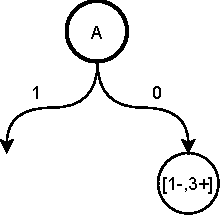
\includegraphics[scale = 0.9]{img/id1.pdf}
  \end{figure}
 \textbf{\textit{Ricordiamo che ID3 sceglie per lo splitting l'attributo che
     rende massimo l'information gain.}}\\
  Passo quindi all'attributo $B$. Si ha che $P_B(0)=\frac{1}{4}$ e
  $P_B(1)=\frac{3}{4}$, quindi:
  \[H[T|B=0]=-p_{T|B}(0|0)\cdot \log_2(p_{T|B}(0|0))-p_{T|B}(1|0)\cdot
    \log_2(p_{T|B}(1|0))=\]
  \[-0\cdot \log_2 0-1\cdot \log_2 1=0\]
  e:
  \[H[T|B=1]=-p_{T|B}(0|1)\cdot \log_2(p_{T|B}(0|1))-p_{T|B}(1|1)\cdot
    \log_2(p_{T|B}(1|1))=\]
  \[-\frac{1}{3}\cdot\log_2\frac{1}{3}-
    \frac{2}{3}\cdot\log_2\frac{2}{3}=0.91\]
  (ho quindi una partizione migliore con $B=0$)\\
  Inoltre si ha:
  \[H[T|B]=P_B(0)\cdot H[T|B=0]+P_B(1)\cdot H[T|B=1]=\frac{1}{4}\cdot
    0+\frac{3}{4}\cdot 0.91=0.68\]
  Posso quindi calcolare l'\textit{information gain}:
  \[IG[T;B]=H[T]-H[T|B]=0.81-0.68=0.13\]
  Quindi per $B$ ho:
  \begin{figure}[H]
    \centering
    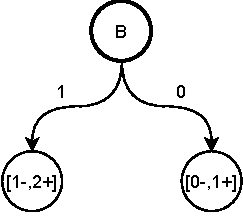
\includegraphics[scale = 0.9]{img/id2.pdf}
  \end{figure}
  Ho quindi un partizionamento più interessante.\\
  Passo quindi all'attributo $C$. Si ha che $P_C(0)=\frac{1}{2}$ e
  $P_C(1)=\frac{1}{2}$, quindi:
  \[H[T|C=0]=-p_{T|C}(0|0)\cdot \log_2(p_{T|C}(0|0))-p_{T|C}(1|0)\cdot
    \log_2(p_{T|C}(1|0))=\]
  \[-\frac{1}{2}\cdot \log_2 \frac{1}{2}-\frac{1}{2}\cdot \log_2 \frac{1}{2}=1\]
  e:
  \[H[T|C=1]=-p_{T|C}(0|1)\cdot \log_2(p_{T|C}(0|1))-p_{T|C}(1|1)\cdot
    \log_2(p_{T|C}(1|1))=\]
  \[-0\cdot \log_2 0-1\cdot \log_2 1=0\]
  Inoltre si ha:
  \[H[T|C]=P_C(0)\cdot H[T|C=0]+P_C(1)\cdot H[T|C=1]=\frac{1}{2}\cdot
    1+\frac{1}{2}\cdot 0=\frac{1}{2}\]
  Posso quindi calcolare l'\textit{information gain}:
  \[IG[T;C]=H[T]-H[T|C]=0.81-\frac{1}{2}=0.31\]
  Quindi per $C$ ho:
  \begin{figure}[H]
    \centering
    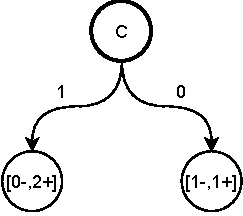
\includegraphics[scale = 0.9]{img/id3.pdf}
  \end{figure}
  $C$ migliora ancora il partizionamento.\\
  Passo quindi all'attributo $D$. Si ha che $P_D(0)=\frac{1}{4}$ e
  $P_D(1)=\frac{3}{4}$, quindi:
  \[H[T|D=0]=-p_{T|D}(0|0)\cdot \log_2(p_{T|D}(0|0))-p_{T|D}(1|0)\cdot
    \log_2(p_{T|D}(1|0))=\]
  \[-1\cdot \log_2 1-0\cdot \log_2 0=0\]
  e:
  \[H[T|D=1]=-p_{T|D}(0|1)\cdot \log_2(p_{T|D}(0|1))-p_{T|D}(1|1)\cdot
    \log_2(p_{T|D}(1|1))=\]
  \[-0\cdot \log_2 0-1\cdot \log_2 1=0\]
  Inoltre si ha:
  \[H[T|D]=P_D(0)\cdot H[T|D=0]+P_D(1)\cdot H[T|D=1]=\frac{1}{4}\cdot
    0+\frac{3}{4}\cdot 0=0\]
  Posso quindi calcolare l'\textit{information gain}:
  \[IG[T;D]=H[T]-H[T|D]=0.81-0=0.81\]
  Quindi per $D$ ho:
  \begin{figure}[H]
    \centering
    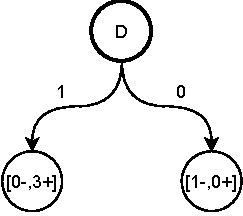
\includegraphics[scale = 0.9]{img/id4.pdf}
  \end{figure}
  $D$ rende quindi il massimo della ``purezza'' tra i valori di $D$ e quelli del
  target. Non si ha incertezza nel partizionamento e non siamo sorpresi da esso.\\
  Quindi, ricapitolando, ho i seguenti information gain:
  \begin{itemize}
    \item $IG[T;A]=0$
    \item $IG[T;B]=0.13$
    \item $IG[T;C]=0.31$
    \item $IG[T;D]=0.81$, \textbf{che è il valore massimo} e che rende minima la
    ``sorpresa''
  \end{itemize}
\end{esempio}
\begin{esempio}
  Considero il seguente training set, con 4 esempi e target $T$:
  \begin{table}[H]
    \centering
    \begin{tabular}{c|c|c|c|c|c}
      example & A & B & C & D & T\\
      \hline
      $x_1$ & 0 & 0 & 1 & $\ldots$ & \color{darkgreen}{1}\\
      $x_2$ & 0 & 1 & 1 & $\ldots$ & \color{darkgreen}{1}\\
      $x_3$ & 0 & 1 & 0 & $\ldots$ & \color{red}{0}\\
      $x_4$ & 0 & 1 & 0 & $\ldots$ & \color{darkgreen}{1}\\
    \end{tabular}
  \end{table}
  Bisogna riempire $D$ per rendere massimo l'information gain.
  \newpage
  Per farlo basta mettere gli stessi valori del target, in modo che sia
  l'attributo che meglio distribuisca i valori del target, ottenendo quindi lo
  stesso training set dell'esempio precedente:
  \begin{table}[H]
    \centering
    \begin{tabular}{c|c|c|c|c|c}
      example & A & B & C & D & T\\
      \hline
      $x_1$ & 0 & 0 & 1 & 1 & \color{darkgreen}{1}\\
      $x_2$ & 0 & 1 & 1 & 1 & \color{darkgreen}{1}\\
      $x_3$ & 0 & 1 & 0 & 0 & \color{red}{0}\\
      $x_4$ & 0 & 1 & 0 & 1 & \color{darkgreen}{1}\\
    \end{tabular}
  \end{table}
  Un'alternativa è l'esatto opposto, in quanto otterrei la stessa
  ridistribuzione del target, rimuovendo ogni ``sorpresa'' ulteriore ma
  lasciando solo quella della tabella iniziale:
  \begin{table}[H]
    \centering
    \begin{tabular}{c|c|c|c|c|c}
      example & A & B & C & D & T\\
      \hline
      $x_1$ & 0 & 0 & 1 & 0 & \color{darkgreen}{1}\\
      $x_2$ & 0 & 1 & 1 & 0 & \color{darkgreen}{1}\\
      $x_3$ & 0 & 1 & 0 & 1 & \color{red}{0}\\
      $x_4$ & 0 & 1 & 0 & 0 & \color{darkgreen}{1}\\
    \end{tabular}
  \end{table}
\end{esempio}
\begin{esempio}
  Considero il seguente training set, con 4 esempi e target $T$:
  \begin{table}[H]
    \centering
    \begin{tabular}{c|c|c|c|c}
      example & $f_1$ & $f_2$ & $f_3$ & T\\
      \hline
      $x_1$ & 1 & 1 & 1 & \color{darkgreen}{1}\\
      $x_2$ & 0 & 1 & 1 & \color{red}{0}\\
      $x_3$ & 0 & 0 & 1 & \color{darkgreen}{1}\\
      $x_4$ & 0 & 0 & 0 & \color{red}{0}\\
    \end{tabular}
  \end{table}
  Vogliamo completare il seguente albero decisionale:
  \begin{figure}[H]
    \centering
    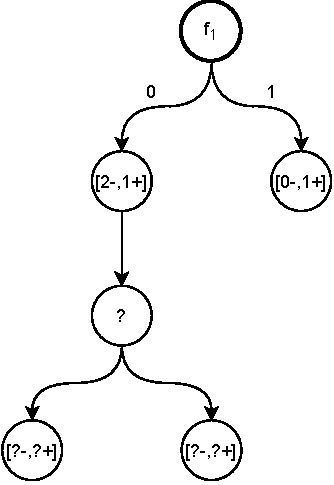
\includegraphics[scale = 0.75]{img/id5.pdf}
  \end{figure}
  Partendo da $f_1$ so che se arriva un nuovo esempio non potrò proseguire da
  $[0-, 1+]$ in quanto so già che in quel caso avrei un'istanza positiva, valore
  minimo $0$.\\
  Quindi se $f_1=0$ vado a scegliere un nuovo attributo in quanto ancora non ho
  una distribuzione certa.\textbf{ Considero quindi le righe in cui $f_1=0$} e avanzo
  iterativamente studiando $f_2$ ed $f_3$. Studio quindi il sottoinsieme: 
  \begin{table}[H]
    \centering
    \begin{tabular}{c|c|c|c}
      example  & $f_2$ & $f_3$ & T\\
      \hline
      $x_2$ & 1 & 1 & \color{red}{0}\\
      $x_3$ & 0 & 1 & \color{darkgreen}{1}\\
      $x_4$ & 0 & 0 & \color{red}{0}\\
    \end{tabular}
  \end{table}
  e avanzo fino a che non finisco gli attributi (o arrivo in un punto in cui,
  come per il ramo 1 di $f_1$ non posso più continuare).\\
  Per questo nuovo sottoinsieme calcolo:
  \[P_T=\left[\frac{2}{3},\frac{1}{4}\right]\]
  e quindi posso calcolare l'entropia della tabella:
  \[H(P_T)=-P_T(0)\cdot \log_2 P_T(0)-P_T(1)\cdot\log_2
    P_T(1)=-\frac{2}{3}\cdot\log_2\frac{2}{3}-\frac{1}{3}\cdot\log_2
    \frac{1}{3}= 0.91\]
  Passo quindi all'attributo $f_2$. Si ha che $P_{f_2}(0)=\frac{2}{3}$ e
  $P_{f_2}(1)=\frac{1}{3}$, quindi:
  \[H[T|f_2=0]=-p_{T|f_2}(0|0)\cdot \log_2(p_{T|f_2}(0|0))-p_{T|f_2}(1|0)\cdot
    \log_2(p_{T|f_2}(1|0))=\]
  \[-\frac{1}{2}\cdot \log_2 \frac{1}{2}-\frac{1}{2}\cdot \log_2 \frac{1}{2}=1\]
  e:
  \[H[T|f_2=1]=-p_{T|f_2}(0|1)\cdot \log_2(p_{T|f_2}(0|1))-p_{T|f_2}(1|1)\cdot
    \log_2(p_{T|f_2}(1|1))=\]
  \[-0\cdot \log_2 0-1\cdot \log_2 1=0\]
  Inoltre si ha:
  \[H[T|f_2]=P_{f_2}(0)\cdot H[T|f_2=0]+P_{f_2}(1)\cdot
    H[T|f_2=1]=\frac{2}{3}\cdot 1+\frac{1}{3}\cdot 0=\frac{2}{3}\]
  Posso quindi calcolare l'\textit{information gain}:
  \[IG[T;f_2]=H[T]-H[T|f_2]=0.81-\frac{2}{3}=0.25\]
  
  Passo quindi all'attributo $f_3$. Si ha che $P_{f_3}(0)=\frac{1}{3}$ e
  $P_{f_3}(1)=\frac{2}{3}$, quindi:
  \[H[T|f_3=0]=-p_{T|f_3}(0|1)\cdot \log_2(p_{T|f_3}(0|1))-p_{T|f_3}(1|1)\cdot
    \log_2(p_{T|f_3}(1|1))=\]
  \[-1\cdot \log_2 1-0\cdot \log_2 0=0\]
  e:
  \[H[T|f_3=1]=-p_{T|f_3}(0|0)\cdot \log_2(p_{T|f_3}(0|0))-p_{T|f_3}(1|0)\cdot
    \log_2(p_{T|f_3}(1|0))=\]
  \[-\frac{1}{2}\cdot \log_2 \frac{1}{2}-\frac{1}{2}\cdot \log_2 \frac{1}{2}=1\]
  Inoltre si ha:
  \[H[T|f_3]=P_{f_3}(0)\cdot H[T|f_3=0]+P_{f_3}(1)\cdot
    H[T|f_3=1]=\frac{1}{3}\cdot 0+\frac{2}{3}\cdot 1=\frac{2}{3}\]
  Posso quindi calcolare l'\textit{information gain}:
  \[IG[T;f_3]=H[T]-H[T|f_3]=0.81-\frac{2}{3}=0.25\]
  Avendo $f_2$ e $f_3$ lo stesso $IG$ prendo il primo e quindi ho:
  \begin{figure}[H]
    \centering
    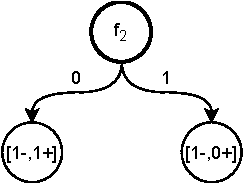
\includegraphics[scale = 0.9]{img/id6.pdf}
  \end{figure}
  Con $f_2$ che verrà attaccato al nodo $[2-, 1+]$ ``uscente'' da $f_1$.\\
 \textbf{ A questo punto, come sopra, abbiamo che il nodo $[1-, 0+]$ è foglia, avendo una
  distribuzione certa}. Riduco quindi nuovamente il training set studiando solo
  gli esempi in cui $f_2$ vale 0, ovvero $x_3$ e $x_4$, per l'attributo $f_3$;
  \begin{table}[H]
    \centering
    \begin{tabular}{c|c|c}
      example & $f_3$ & T\\
      \hline
      $x_3$ & 1 & \color{darkgreen}{1}\\
      $x_4$ & 0 & \color{red}{0}\\
    \end{tabular}
  \end{table}
  \newpage
  Non sono necessari conti in quanto $f_3$ è l'ultimo attributo rimasto ed è
  distribuito in questo modo:
  \begin{figure}[H]
    \centering
    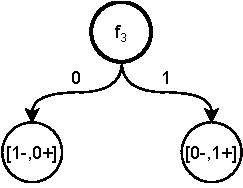
\includegraphics[scale = 0.9]{img/id7.pdf}
  \end{figure}
  Avendo per di più entrambi i risultati con distribuzione certa.\\
  Il nodo di $f_3$ sarà attaccato al nodo $[1-, 1+]$ ``uscente'' da $f_2$,
  ottenendo così l'albero:
  \begin{figure}[H]
    \centering
    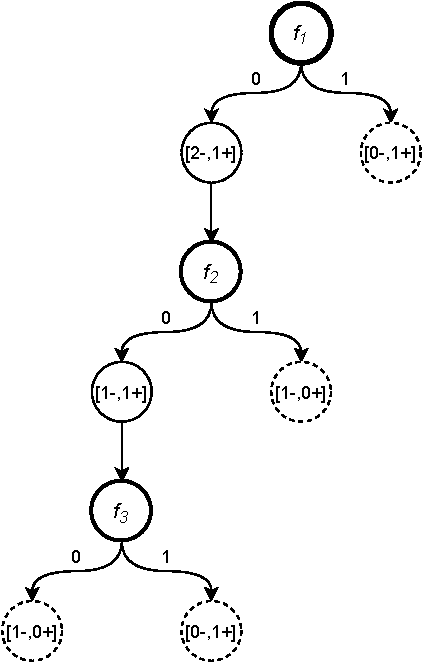
\includegraphics[scale = 1]{img/id8.pdf}
  \end{figure}
\end{esempio}
% \section{Considerazioni Finali}
% Arrivati a questo punto è necessario fare un resoconto finale su come costruire un albero partendo da un Training Set.
% \begin{enumerate}
%     \item Calcolo dell'entropia del Training Set (\ref{Contenuto informatico di un insieme} o \ref{Contenuto informativo di un training set}):
%     \[I\left(\frac{p}{p+n},\frac{n}{p+n}\right)=-\frac{p}{p+n}\log_2\frac{p}{p+n}
%     -\frac{n}{p+n}\log_2\frac{n}{p+n}\]
    
%     \item Calcolo delle probabilità del primo attributo in tabella disponibile:
%     \[\frac{p_i+n_i}{p+n}\]

%     \item Calcolo l'entropia/contenuto informativo dell'attributo:
%         \begin{enumerate}
%             \item In Generale avremo:
%             \[I\left(\frac{p_i}{p_i+n_i},\frac{n_i}{p_i+n_i}\right)\]
            
%             \item Se si parla di probabilità condizionata, dalla precedente formula si deriva:
%             \[I_{Y|X=x_i}=-\sum_{j=1}^m P_{Y|X}(y_j|x_i)\cdot \log_2 P_{Y|X}(y_j|x_i)\]
%         \end{enumerate}
    
%     \item Calcolo il $Resto(A)$
%         \begin{enumerate}
%           \item In generale si opta per:
%             \[remainder(A)=\sum_{i=1}^v \frac{p_i+n_i}{p+n}
%   I\left(\frac{p_i}{p_i+n_i},\frac{n_i}{p_i+n_i}\right)\]
          
%             \item In caso di probabilità condizionata la formula si riduce alla \ref{EntropiaCondizionale}:
%                   \[H[Y|X]=\sum P(x)\cdot H(Y|X=x)\]
%         \end{enumerate}
          
%     \item Calcolo IG :
%             \[IG(S,A)=I\left(\frac{p}{p+n},\frac{n}{p+n}\right)-remainder(A)\]
% \end{enumerate}

